\documentclass[conference]{IEEEtran}
\usepackage{cite}
\usepackage{amsmath,amssymb}
\usepackage{graphicx}
\usepackage{booktabs}
\usepackage{siunitx}
\usepackage{xcolor}
\usepackage[hidelinks]{hyperref}
\graphicspath{{../../outputs/figures/}}
\newcommand{\NTracts}{9,794}
\newcommand{\NHU}{17.1}
\newcommand{\NPop}{41.8}
\newcommand{\NBldg}{19.2}
\newcommand{\NPoi}{2.0}
\newcommand{\RefCorr}{0.975}
\newcommand{\RefMedRatio}{1.05}
\newcommand{\RefGapShare}{1.9\%}
\newcommand{\RefGapRural}{4.7\%}
\newcommand{\RefGapUrban}{1.3\%}
\newcommand{\RefGapTribal}{4.3\%}
\newcommand{\RefGapNonTribal}{1.6\%}
\newcommand{\CovBldg}{90.0\%}
\newcommand{\CovPoi}{90.0\%}
\newcommand{\FlagBldg}{510}
\newcommand{\FlagPoi}{529}
\newcommand{\RTwoBldg}{0.93}
\newcommand{\RTwoPoi}{0.82}
\newcommand{\CovSpatRegMinBldg}{88.9\%}
\newcommand{\CovSpatRegMaxBldg}{93.2\%}
\newcommand{\CovMondRegMinBldg}{88.9\%}
\newcommand{\CovMondRegMaxBldg}{90.2\%}
\newcommand{\CovLoroBldg}{84.6\%}
\newcommand{\CovLoroMinBldg}{78.1\%}
\newcommand{\PrecBldg}{0.09}
\newcommand{\RecBldg}{0.26}
\newcommand{\PrevBldg}{1.9\%}
\newcommand{\LiftBldg}{5.1}
\newcommand{\PRAUCBldg}{0.10}
\newcommand{\PRAUCOlsBldg}{0.06}
\newcommand{\PRAUCRatioBldg}{0.08}
\newcommand{\PrecPoi}{0.58}
\newcommand{\PrevPoi}{24.0\%}
\newcommand{\DelThirtyBldg}{66\%}
\newcommand{\DelFiftyBldg}{96\%}
\newcommand{\DelThirtyPoi}{18\%}
\newcommand{\DelFiftyPoi}{56\%}
\newcommand{\CountyRho}{0.85}
\newcommand{\CountyN}{324}
\newcommand{\NFdrFamily}{25}
\newcommand{\PoiSviHi}{3.8\%}
\newcommand{\PoiSviLo}{8.9\%}
\newcommand{\PoiSviAor}{0.41}
\newcommand{\HFiveWildRural}{4.8}
\newcommand{\HFiveWildRuralCI}{[2.4, 9.4]}
\newcommand{\HFiveDroughtRural}{2.9}
\newcommand{\HFiveDroughtRuralCI}{[1.2, 7.1]}
\newcommand{\HFiveHeatTribal}{0.08}
\newcommand{\HFiveHeatTribalCI}{[0.0, 0.4]}
\newcommand{\HEAll}{44,945}
\newcommand{\HFourDprBldg}{-0.010}
\newcommand{\HFourDprBldgCI}{[-0.035, +0.016]}
\newcommand{\HFourDaucPoi}{+0.004}
\newcommand{\HFourDaucPoiCI}{[+0.001, +0.007]}
\newcommand{\GapMsft}{2.8\%}
\newcommand{\GapOsm}{1.3\%}
\newcommand{\GainBldg}{1.7}
\newcommand{\OsmShareA}{31\%}
\newcommand{\OsmShareC}{51\%}
\newcommand{\GapShareA}{7.0\%}
\newcommand{\GapShareB}{1.8\%}
\newcommand{\GapRuralA}{15.7\%}
\newcommand{\GapRuralC}{4.2\%}
\newcommand{\GapSviC}{5.3\%}
\newcommand{\DidRuralPP}{9.9}
\newcommand{\DidRuralCI}{[-15.3, -5.5]}
\newcommand{\DidRuralP}{0.003}
\newcommand{\DidTribalPP}{6.7}
\newcommand{\DidTribalCI}{[-14.3, -0.6]}
\newcommand{\DidTribalP}{0.061}
\newcommand{\HThreeRural}{$+$0.060 log points, 95\% CI 0.013--0.106}
\newcommand{\HThreeRuralP}{0.040}
\newcommand{\EOneLost}{179,000}
\newcommand{\EOneTracts}{186}
\newcommand{\EOneBexar}{181}
\newcommand{\EOneResidents}{889,000}
\newcommand{\EOneSviShare}{63\%}
\newcommand{\EOneSviAll}{34\%}
\newcommand{\EOneFlagAfter}{82\%}
\newcommand{\EOneFlagBefore}{2.7\%}
\newcommand{\EOneFlagOther}{4.5\%}
\newcommand{\EOneRecall}{83\%}
\newcommand{\EOneRefGapAfter}{99\%}
\newcommand{\EThreeSummary}{rural +0.034 (endpoint 2026-08-19; 95\% CI 0.003--0.065); rural +0.040 (excluding Bexar County; 95\% CI 0.008--0.072); tribal +0.035 (endpoint 2026-08-19; 95\% CI 0.004--0.067); tribal +0.036 (excluding Bexar County; 95\% CI 0.002--0.070)}
\newcommand{\ETwoText}{For rural vs.\ urban tracts the adjusted odds ratio of a reference gap is 3.86 [2.40, 6.22], but 1.06 [0.72, 1.57] for the map-trained flag and 0.83 [0.48, 1.44] for the reference-anchored flag; for tribal vs.\ non-tribal tracts the values are 4.17 [1.89, 9.23], 1.26 [0.38, 4.20] and 0.92 [0.17, 5.14]. \emph{Absorption} is visible in the expectation itself: relative to the reference, observed completeness in rural tracts is lower by -0.031 [-0.053, -0.009] log points (region FE), and the map-trained expectation is already lower by -0.025 [-0.053, 0.004], so it reproduces 80\% of the rural shortfall (64\% of the tribal one). \emph{Resolution} limits even the reference-anchored model: its tract-level residual SD is 0.21 log points (map-trained: 0.19), against 0.22 for a 20\% gap, and it flags only 2.3\% of tracts (precision 0.16, recall 0.20 for reference gaps; map-trained 0.09 and 0.26).}
\newcommand{\OrigHOne}{4.9 vs.\ 2.3}
\newcommand{\OrigHOneP}{0.0004}
\newcommand{\RobustText}{Across 7 specifications (primary; no housing-type covariates; negative-binomial GLM; 80\% and 95\% ranges; within-region calibration; excluding tracts with fewer than 50 housing units), 53 of 56 flag contrasts keep the significance status of the primary analysis. The lower POI flag rate in high-SVI tracts holds in every specification (risk difference -0.040 to -0.067). The exceptions are: no housing-type covariates, building svi: RD +0.059 [+0.025, +0.086]; negative-binomial GLM, POI rural: RD -0.010 [-0.024, +0.002]; 95\% range, POI tribal: RD -0.012 [-0.028, -0.002]. Most notably, dropping units-in-structure covariates makes building flags significantly more common in high-SVI tracts (aOR 2.91), consistent with absorption: mobile-home and multi-unit housing shares, which correlate with SVI, explain away part of the high-SVI shortfall in the primary model. Details are in Appendix Table~\ref{tab:robust}.}
\newcommand{\RobustTextShort}{Across 7 specifications (primary; no housing-type covariates; negative-binomial GLM; 80\% and 95\% ranges; within-region calibration; excluding tracts with fewer than 50 housing units), 53 of 56 flag contrasts keep the significance status of the primary analysis. The lower POI flag rate in high-SVI tracts holds in every specification (risk difference -0.040 to -0.067). The exceptions are: no housing-type covariates, building svi: RD +0.059 [+0.025, +0.086]; negative-binomial GLM, POI rural: RD -0.010 [-0.024, +0.002]; 95\% range, POI tribal: RD -0.012 [-0.028, -0.002]. Most notably, dropping units-in-structure covariates makes building flags significantly more common in high-SVI tracts (aOR 2.91), consistent with absorption: mobile-home and multi-unit housing shares, which correlate with SVI, explain away part of the high-SVI shortfall in the primary model. Full results are in \texttt{outputs/tables/robustness.csv}.}

% generated by scripts/12_merged_numbers.py -- do not edit
\newcommand{\MgRegTracts}{186}
\newcommand{\MgRegBexar}{181}
\newcommand{\MgRegMsftPooled}{79.5\%}
\newcommand{\MgRegMsftMean}{78.6\%}
\newcommand{\MgSctxMsftMean}{37.5\%}
\newcommand{\MgRegDom}{44\%}
\newcommand{\MgSctxDom}{19\%}
\newcommand{\MgRegDomDiff}{25}
\newcommand{\MgRegDomCICounty}{[-23, 31]}
\newcommand{\MgRegDomCITract}{[18, 32]}
\newcommand{\MgRegClass}{4.1\%}
\newcommand{\MgSctxClass}{25.4\%}
\newcommand{\MgRegSpearman}{0.68}
\newcommand{\MgRegLossLeMsft}{100\%}
\newcommand{\MgDomTracts}{1,854}
\newcommand{\MgDomTractShare}{19\%}
\newcommand{\MgDomPop}{7.33}
\newcommand{\MgDomLabel}{1.0\%}
\newcommand{\MgOtherLabel}{24.9\%}
\newcommand{\MgDomHeight}{75\%}
\newcommand{\MgOtherHeight}{75\%}
\newcommand{\MgDomRural}{40\%}
\newcommand{\MgOtherRural}{12\%}
\newcommand{\MgDomTribal}{23\%}
\newcommand{\MgOtherTribal}{6\%}
\newcommand{\MgDomGap}{2.9\%}
\newcommand{\MgOtherGap}{1.6\%}
\newcommand{\MgClassAUC}{0.56}
\newcommand{\MgClassAUCCI}{[0.48, 0.65]}
\newcommand{\MgClassOR}{3.3}
\newcommand{\MgClassORCI}{[1.2, 9.2]}
\newcommand{\MgClassPbh}{0.12}
\newcommand{\MgNFam}{64}
\newcommand{\MgBudget}{510}
\newcommand{\MgLiftIF}{5.3}
\newcommand{\MgLiftNB}{5.1}
\newcommand{\MgLiftRatio}{4.9}
\newcommand{\MgLiftMin}{4.0}
\newcommand{\MgLiftMax}{5.3}
\newcommand{\MgXgbAucDiff}{+0.04}
\newcommand{\MgXgbAucDiffCI}{[0.00, 0.09]}
\newcommand{\MgRatioAucDiff}{-0.22}
\newcommand{\MgRatioAucDiffCI}{[-0.33, -0.14]}
\newcommand{\MgGERecall}{0.000}
\newcommand{\MgGERecallCI}{[-0.027, 0.036]}
\newcommand{\MgDroughtWithin}{1.65}
\newcommand{\MgDroughtWithinCI}{[0.74, 3.27]}
\newcommand{\MgWildMin}{3.80}
\newcommand{\MgWildMax}{6.25}
\newcommand{\MgRrmseBldg}{0.49}
\newcommand{\MgRrmseHwy}{0.52}
\newcommand{\MgRrmseFire}{0.92}
\newcommand{\MgRrmseEms}{0.99}
\newcommand{\MgHwyLoroAz}{1.42}
\newcommand{\MgHwyLoroTx}{0.70}
\newcommand{\MgProvMaeMin}{+0.002}
\newcommand{\MgProvMaeMax}{+0.006}
\newcommand{\MgReproCols}{111}
\newcommand{\MgReproColsTotal}{111}
\newcommand{\MgBoundaryPlaces}{59}
\newcommand{\MgImgFirst}{2006}
\newcommand{\MgImgLast}{2021}
\newcommand{\MgSeedOverlap}{0.73}
\newcommand{\MgSeedChanged}{27\%}
\newcommand{\MgNVariants}{17}
\newcommand{\MgSettingsOverlapMin}{0.65}
\newcommand{\MgSettingsOverlapMax}{0.90}
\newcommand{\MgCovMin}{89.9\%}
\newcommand{\MgCovMax}{90.1\%}
\newcommand{\MgRTwoPrim}{0.926}
\newcommand{\MgRTwoNoHt}{0.845}
\newcommand{\MgLiftNoHt}{3.6}
\newcommand{\MgOverlapNoHt}{0.27}
\newcommand{\MgFlagSmallDecile}{14\%}
\newcommand{\MgFlagLargeDecile}{1\%}
\newcommand{\MgWaFlag}{0.2\%}
\newcommand{\MgWaAbove}{11\%}
\newcommand{\MgReproFlags}{9,794}
\newcommand{\MgReproFlagsTotal}{9,794}
\newcommand{\MgUnassignedBldg}{3}
\newcommand{\MgRawBldg}{19,169,789}
\newcommand{\MgUnassignedPoi}{62}
\newcommand{\MgRawPoi}{2,001,137}
\newcommand{\MgGqTracts}{101}
\newcommand{\MgMoranMin}{0.09}
\newcommand{\MgMoranMax}{0.18}

% generated by scripts/14_reference_validation.py -- do not edit
\newcommand{\RvMeAuc}{0.77}
\newcommand{\RvMeAucCI}{[0.71, 0.83]}
\newcommand{\RvMeRho}{0.24}
\newcommand{\RvMeRhoCI}{[0.18, 0.30]}
\newcommand{\RvMeLift}{3.01}
\newcommand{\RvMeLiftCI}{[2.43, 3.56]}
\newcommand{\RvCfAuc}{0.68}
\newcommand{\RvCfAucCI}{[0.62, 0.74]}
\newcommand{\RvCfRho}{0.17}
\newcommand{\RvCfRhoCI}{[0.13, 0.22]}
\newcommand{\RvCfLift}{2.38}
\newcommand{\RvCfLiftCI}{[1.85, 2.83]}
\newcommand{\RvRawAuc}{0.44}
\newcommand{\RvRawAucCI}{[0.31, 0.55]}
\newcommand{\RvRawRho}{0.03}
\newcommand{\RvRawRhoCI}{[-0.08, 0.10]}
\newcommand{\RvRawLift}{1.49}
\newcommand{\RvRawLiftCI}{[0.68, 2.25]}
\newcommand{\RvMeRiskAuc}{0.67}
\newcommand{\RvMeRiskAucCI}{[0.59, 0.76]}
\newcommand{\RvMeRiskRho}{0.11}
\newcommand{\RvMeRiskRhoCI}{[0.07, 0.17]}
\newcommand{\RvMeRiskLift}{2.29}
\newcommand{\RvMeRiskLiftCI}{[1.67, 2.94]}
\newcommand{\RvPairDiff}{+0.087}
\newcommand{\RvPairCI}{[+0.035, +0.146]}
\newcommand{\RvRuralMe}{1.25}
\newcommand{\RvRuralMeCI}{[1.06, 1.44]}
\newcommand{\RvRuralCf}{1.00}
\newcommand{\RvRuralCfCI}{[0.80, 1.24]}
\newcommand{\RvRuralRef}{3.72}
\newcommand{\RvRuralRefCI}{[2.19, 7.12]}
\newcommand{\RvTribalMe}{1.49}
\newcommand{\RvTribalMeCI}{[1.22, 1.88]}
\newcommand{\RvTribalCf}{0.99}
\newcommand{\RvTribalCfCI}{[0.59, 1.35]}
\newcommand{\RvTribalRef}{2.71}
\newcommand{\RvTribalRefCI}{[1.21, 5.71]}
\newcommand{\RvFlagAzRur}{11.6\%}
\newcommand{\RvRefAzRur}{2.3\%}
\newcommand{\RvFlagAzUrb}{3.5\%}
\newcommand{\RvRefAzUrb}{0.8\%}
\newcommand{\RvFlagOkRur}{2.8\%}
\newcommand{\RvRefOkRur}{7.7\%}
\newcommand{\RvFlagOkUrb}{4.6\%}
\newcommand{\RvRefOkUrb}{0.9\%}
\newcommand{\RvN}{9,788}

% generated by scripts/15_journal_checks.py -- do not edit
\newcommand{\JoFlagRate}{5.1\%}
\newcommand{\JoTwoBelow}{5.2\%}
\newcommand{\JoTwoAbove}{4.8\%}
\newcommand{\JoJaccard}{0.98}
\newcommand{\JoLift}{5.1}
\newcommand{\JoPrec}{0.095}
\newcommand{\JoRegMin}{0.2\%}
\newcommand{\JoRegMax}{5.9\%}
\newcommand{\JsPairMin}{0.71}
\newcommand{\JsPairMax}{0.76}
\newcommand{\JsPairMean}{0.74}
\newcommand{\JsEver}{750}
\newcommand{\JsStable}{375}
\newcommand{\JsMajority}{486}
\newcommand{\JsSingleLift}{5.0}
\newcommand{\JsStableLift}{6.3}
\newcommand{\JsStablePrec}{0.116}
\newcommand{\JsStableRecall}{0.238}
\newcommand{\JsMajLift}{5.5}
\newcommand{\JtGlobalMin}{77.6\%}
\newcommand{\JtGlobalMax}{94.4\%}
\newcommand{\JtFiftyMin}{90.0\%}
\newcommand{\JtFiftyMax}{90.4\%}
\newcommand{\JtFiftyLo}{82.6\%}
\newcommand{\JtFiftyHi}{96.4\%}
\newcommand{\JhWildfireRural}{13.84}
\newcommand{\JhWildfireRuralCI}{[7.92, 22.04]}
\newcommand{\JhWildfireTribal}{9.72}
\newcommand{\JhWildfireTribalCI}{[4.70, 19.07]}
\newcommand{\JhDroughtRural}{4.89}
\newcommand{\JhDroughtRuralCI}{[2.60, 12.45]}
\newcommand{\JhDroughtTribal}{1.95}
\newcommand{\JhDroughtTribalCI}{[0.85, 4.19]}
\newcommand{\JhHeatRural}{2.25}
\newcommand{\JhHeatRuralCI}{[0.99, 7.36]}
\newcommand{\JhHeatTribal}{0.06}
\newcommand{\JhHeatTribalCI}{[0.01, 0.20]}
\newcommand{\JhMissTotal}{300,495}
\newcommand{\JmGlmAuc}{0.75}
\newcommand{\JmGlmPr}{0.063}
\newcommand{\JmLgbAuc}{0.69}
\newcommand{\JmLgbPr}{0.137}
\newcommand{\JmCfPr}{0.099}
\newcommand{\JmMePr}{0.070}
\newcommand{\JmGlmTop}{0.090}
\newcommand{\JmLgbTop}{0.135}
\newcommand{\JrRuralSeven}{3.51}
\newcommand{\JrRuralNine}{3.07}
\newcommand{\JrOrderHolds}{holds}


\begin{document}
\title{Invisible Exposure: Reference-Free Conformal Detection of Missing Buildings in Open Maps and the Climate Risk They Hide}

\author{\IEEEauthorblockN{Pradeep T, Prajwal A, Nikhita P Uppar, Sakshi Kiran}
\IEEEauthorblockA{Department of Computer Science and Engineering (AI \& ML), PES University, Bengaluru, India\\
ADA Course Project $\cdot$ Code, data and notebook: \url{https://github.com/GTX-Pradeep/invisible-exposure-open-map-equity}}}

\maketitle

\begin{abstract}
Climate-risk tools estimate exposure by overlaying hazard layers on building maps, so a building that is missing from the map is missing from the exposure count. Finding such gaps normally requires a complete reference map, which rarely exists. We test whether open-map gaps can be detected without one. From neutral structural facts alone (housing stock, population, land area and jobs), we predict how many buildings and points of interest each of \NTracts{} census tracts should contain, and we wrap each prediction in a calibrated range using cross-fitted conformalized quantile regression. A tract is flagged when the map falls below its range. Vulnerability, rurality, tribal status and hazard severity are blocked from the model in code and are used only in an analysis registered before any result was examined. The ranges cover \CovBldg{} of held-out tracts at a 90\% target, falling to \CovLoroBldg{} when a whole region is held out. Against FEMA/ORNL USA Structures, flagged tracts are \LiftBldg{}$\times$ more likely than chance to be real gaps, and deleting half of a tract's buildings triggers a flag \DelFiftyBldg{} of the time. Across three Overture releases, rural gaps closed \DidRuralPP{} percentage points faster than urban ones. We also document a silent release regression: from 23 September 2026, Overture dropped about \EOneLost{} buildings from \EOneTracts{} tracts around San Antonio, and the model, which uses no reference, flagged \EOneFlagAfter{} of them. Finally, we show that per-tract flags cannot detect a modest gap shared by a whole group.
\end{abstract}

\begin{IEEEkeywords}
open map data, Overture Maps, conformal prediction, data completeness, environmental justice, climate risk
\end{IEEEkeywords}

\section{Introduction}
A climate-risk estimate is only as good as the map beneath it. Counting the homes a wildfire threatens usually means overlaying a burn-probability layer on a building map. A house that is not on the map is not counted, and its neighbourhood appears safer, and less in need of support, than it is.

If maps were incomplete uniformly, this would matter less. Open map coverage, however, is thinner in poorer and more rural places \cite{haklay2010,mashhadi2013,herfort2023}, so the undercount is likely to be largest where the stakes are highest.

Measuring this undercount normally requires a more complete map to compare against, and for most regions and feature types no such map exists. Counting sparse tracts does not help either: a tract with few mapped buildings may be farmland, or it may be an unmapped suburb.

\textbf{What we do.} We estimate where Overture Maps \cite{overture} is incomplete at census-tract level without consulting a reference at prediction time. We attach a calibrated range to every estimate, convert the gaps into hidden heat, wildfire and drought exposure, and test, under a pre-registered plan, whether the gaps fall on vulnerable, rural and tribal communities and whether they are closing.

\textbf{Contributions.} (i) A completeness model that cannot see the variables it is later audited on, with calibrated per-tract ranges and a study of how that calibration survives being moved across space. (ii) Validation against two independent references plus a controlled deletion test. (iii) A three-release audit that uncovered a silent release regression. (iv) Pre-registered equity and hidden-exposure contrasts with false-discovery-rate control. (v) An account of why per-tract flags miss group-wide gaps, which is a limit of the approach rather than of the implementation.

\section{Related Work}
Studies of OpenStreetMap completeness have tied coverage to population density and affluence \cite{haklay2010,thebaultspieker2018}, and POI coverage specifically to deprivation \cite{mashhadi2013}. The closest work is Herfort et al. \cite{herfort2023}, who estimate global building completeness by regression, but as point estimates, without a statement of how wrong any single estimate could be.

Conformal prediction provides such a statement, with finite-sample coverage under exchangeability \cite{vovk2005,lei2018}, and conformalized quantile regression (CQR) lets the interval width follow the noise \cite{romano2019}. Two findings from this literature shaped our design: coverage can degrade under distribution shift \cite{tibshirani2019}, and random cross-validation overstates spatial accuracy by splitting neighbours across folds \cite{roberts2017}. We therefore compare three fold schemes. In addition, a model fitted to biased outcomes reproduces the bias \cite{obermeyer2019}. Our model learns from the map it audits, so it shares this risk, and Section~\ref{sec:lens} measures how much of the bias it inherits.

\section{Data}
\subsection{The Open Map Equity challenge}
The study area, the map snapshots and the audit strata all come from the \emph{Bias Bounty: Mapping Equity} challenge (the Open Map Equity challenge) run by Humane Intelligence with Zindi \cite{biasbounty}. It publishes map extracts and a curated set of social, demographic and hazard strata for five U.S. regions selected for their climate exposure: Maricopa County AZ, northern CA, eastern OK, south-central TX and eastern WA. Together these hold \NTracts{} census tracts, \NHU{}M housing units and \NPop{}M residents.

Using the challenge regions provides strata assembled for this purpose and keeps our work comparable with other submissions. It also bounds generalisation, because five hazard-selected regions are not a national sample.

Our task differs from the challenge's. The challenge scores gaps against references that it supplies. We predict expected counts with no reference in the loop, attach a calibrated range to every tract, span three releases rather than one, and fix the equity hypotheses before seeing results.

\subsection{Map, inputs and references}
The map under audit is Overture \texttt{2026-08-19.0}: \NBldg{}M buildings and \NPoi{}M places across the five regions. We add \texttt{2026-10-21.0} and an archived copy of \texttt{2023-07-26-alpha.0} to follow change over time. Features are assigned to tracts by bounding-box centre, and only buildings of at least 450\,sq\,ft are counted so that counts match the reference.

The model is restricted to four kinds of input: housing and population counts; units in structure and year built, from the 2020--2024 ACS \cite{acs}; tract land area; and 2022 LODES jobs by sector \cite{lodes}. No other variable is made available to it.

Two references are held back for validation and never shown to the model: FEMA/ORNL USA Structures \cite{usastructures} for buildings, and ZIP and County Business Patterns \cite{cbp} for establishments. The audit strata (SVI 2022 \cite{flanagan2011}, CVI, RUCA rurality, tribal-land overlap, EPHT heat days, USFS burn probability \cite{wrc} and USDM drought) are joined only after the model has finished predicting.

Each Overture release is several gigabytes, and three were needed. DuckDB with its spatial and httpfs extensions reads the cloud GeoParquet directly and fetches only the row groups that intersect the study regions, so no release is downloaded in full.

\section{Method}
\subsection{Expected counts}
For tract $i$ with mapped count $c_i$ we model $y_i=\log(1+c_i)$ on structural covariates $x_i$. Three LightGBM \cite{ke2017} quantile regressions estimate $\hat q_\tau(x)$ at $\tau\in\{0.05,0.5,0.95\}$. A guard, \texttt{assert\_no\_leakage}, rejects any audit, reference or outcome column at fit time, so the exclusion is enforced by the pipeline.

Predictions are cross-fitted over $K=10$ folds built from whole \SI{50}{km} spatial blocks. With random folds, a tract's own deficit, which it shares with its neighbours, would lower the expectation against which it is judged; spatial blocks prevent this.

\subsection{Calibrated ranges}
Out-of-fold CQR scores $s_i=\max\{\hat q_{0.05}(x_i)-y_i,\,y_i-\hat q_{0.95}(x_i)\}$ record how badly each interval missed. For fold $k$, the correction $\hat Q_k$ is the $\lceil 0.9(m+1)\rceil$-th smallest of the $m$ scores from the other folds, giving $[\hat q_{0.05}-\hat Q_k,\ \hat q_{0.95}+\hat Q_k]$. A Mondrian variant computes $\hat Q_k$ within each region. A tract is flagged when $y_i$ sits below the lower bound; its shortfall is the conservative $\max(\text{lower}-c_i,0)$.

Cross-fitted CQR is a CV+-type procedure, so its worst-case guarantee is $1-2\alpha$, not exactly $1-\alpha$. The measured coverage is close to nominal, but the theory does not guarantee this.

\subsection{Validation and pre-registration}
We compare random, spatial-block and leave-one-region-out folds; score flags against reference gaps (Overture below 80\% of USA Structures); and run a deletion test that removes a known share of a tract's features and checks whether the model flags the tract.

Hypotheses were frozen before any model output was joined to any stratum. H1 and H2 test flag rates by SVI, CVI, rurality and tribal status, using logistic regression with region fixed effects, county-clustered standard errors and a cluster bootstrap over 324 counties. H3 tests catch-up from 2023 to 2026. H4 tests whether data-provenance features improve detection. H5 tests hidden exposure per 1,000 housing units in top-tercile hazard tracts. Benjamini--Hochberg control \cite{bh1995} is applied across all \NFdrFamily{} tests. Everything outside that family is labelled exploratory.

\section{Results}
\subsection{Calibration}
Overture and USA Structures agree closely (log $r=\RefCorr{}$, median ratio 1.05); only \RefGapShare{} of tracts hold less than 80\% of the reference: \RefGapRural{} rural and \RefGapTribal{} tribal, against \RefGapUrban{} urban and \RefGapNonTribal{} non-tribal. Spatial cross-fitting reaches $R^2=\RTwoBldg{}$ for buildings and \RTwoPoi{} for POIs, at \CovBldg{} coverage on both layers.

Where the calibration is computed matters more than how folds are drawn (Table~\ref{tab:cv}, Fig.~\ref{fig:cov}). Under one global calibration, per-region coverage spans \CovSpatRegMinBldg{}--\CovSpatRegMaxBldg{}; calibrating within each region narrows it to \CovMondRegMinBldg{}--\CovMondRegMaxBldg{}. Holding out a whole region lowers coverage to \CovLoroBldg{}, and to \CovLoroMinBldg{} in one region. This is a real limit on transfer, but it can be repaired: recalibrating on 50 tracts of the held-out region, which needs only the map's own counts, restores \JtFiftyMin{}--\JtFiftyMax{}.

\begin{table}[t]\centering\footnotesize
\caption{Calibration and fit by fold scheme. Coverage is of nominal 90\% ranges; $R^2$ is on the log scale; the last columns are per-region coverage extremes.}\label{tab:cv}
\resizebox{\columnwidth}{!}{\begin{tabular}{lllrrrrr}
\toprule
Layer & Folds & Calibration & Coverage \% & Flags \% & $R^2$ & Region min & Region max \\
\midrule
bldg & random & global & 90.0 & 5.2 & 0.930 & 88.9 & 93.1 \\
bldg & random & mondrian-region & 90.0 & 5.2 & 0.930 & 89.8 & 90.1 \\
bldg & spatial & global & 90.0 & 5.2 & 0.926 & 88.9 & 93.2 \\
bldg & spatial & mondrian-region & 90.0 & 5.2 & 0.926 & 88.9 & 90.2 \\
bldg & region & global & 84.6 & 8.9 & 0.904 & 78.1 & 96.8 \\
bldg & region & mondrian-region & 84.6 & 8.9 & 0.904 & 78.1 & 96.8 \\
poi & random & global & 90.0 & 5.5 & 0.830 & 87.0 & 92.4 \\
poi & random & mondrian-region & 90.1 & 5.5 & 0.830 & 89.9 & 90.2 \\
poi & spatial & global & 90.0 & 5.4 & 0.824 & 85.3 & 93.4 \\
poi & spatial & mondrian-region & 89.9 & 5.4 & 0.824 & 89.7 & 90.1 \\
poi & region & global & 88.1 & 4.9 & 0.806 & 85.4 & 96.3 \\
poi & region & mondrian-region & 88.1 & 4.9 & 0.806 & 85.4 & 96.3 \\
\bottomrule
\end{tabular}}
\end{table}

\begin{figure}[t]\centering
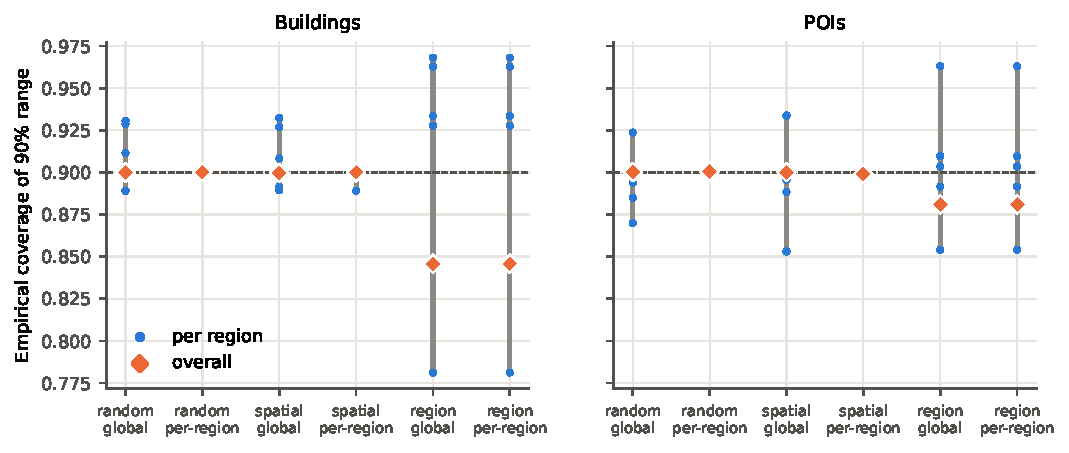
\includegraphics[width=\columnwidth]{fig3_coverage_schemes.pdf}
\caption{Coverage of nominal 90\% ranges by fold scheme and calibration. Dots are regions, diamonds the overall value.}\label{fig:cov}
\end{figure}

\subsection{Do the flags find real gaps?}
Against USA Structures the building flags reach precision \PrecBldg{} and recall \RecBldg{} at \PrevBldg{} prevalence, a lift of \LiftBldg{}$\times$, with PR-AUC \PRAUCBldg{} against \PRAUCOlsBldg{} for an OLS baseline and \PRAUCRatioBldg{} for a map-to-housing ratio (Table~\ref{tab:skill}).

The precision is low in absolute terms because real gaps are rare. The deletion test gives cleaner evidence, because the gap is known: removing 30\% of a tract's buildings triggers a flag \DelThirtyBldg{} of the time, and removing 50\% triggers one \DelFiftyBldg{} of the time (Fig.~\ref{fig:del}). The POI layer is less sensitive (\DelThirtyPoi{} and \DelFiftyPoi{}).

\begin{table}[t]\centering\footnotesize
\caption{Flag skill against the independent references.}\label{tab:skill}
\resizebox{\columnwidth}{!}{\begin{tabular}{llrrrrrrrr}
\toprule
Layer & Method & $n$ & Prev. & Flags & Prec. & Recall & Lift & ROC-AUC & PR-AUC \\
\midrule
Buildings & conformal model & 9,793 & 1.9\% & 510 & 0.094 & 0.264 & 5.1 & 0.685 & 0.099 \\
Buildings & OLS log-HU & 9,793 & 1.9\% & 510 & 0.075 & 0.209 & 4.0 & 0.727 & 0.060 \\
Buildings & map/housing ratio & 9,793 & 1.9\% & 510 & 0.090 & 0.253 & 4.9 & 0.463 & 0.081 \\
POIs & conformal model & 9,309 & 24.0\% & 495 & 0.584 & 0.130 & 2.4 & 0.671 & 0.415 \\
POIs & OLS log-HU & 9,309 & 24.0\% & 495 & 0.699 & 0.155 & 2.9 & 0.780 & 0.535 \\
POIs & map/housing ratio & 9,309 & 24.0\% & 495 & 0.675 & 0.150 & 2.8 & 0.764 & 0.514 \\
\bottomrule
\end{tabular}}
\end{table}

\begin{figure}[t]\centering
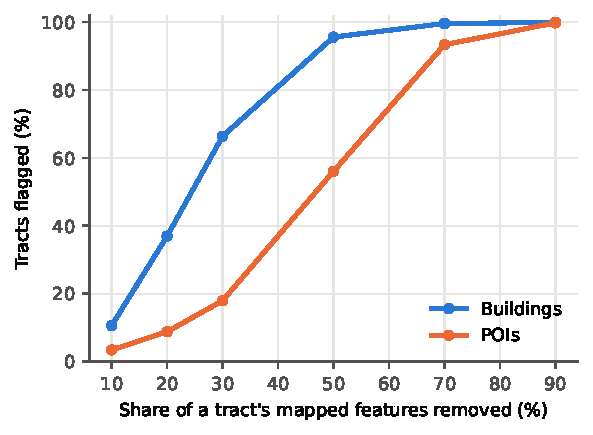
\includegraphics[width=0.8\columnwidth]{fig4_deletion.pdf}
\caption{Deletion test: share of tracts flagged after a known share of their features is removed.}\label{fig:del}
\end{figure}

\subsection{Who the gaps fall on, and the exposure they hide}
Table~\ref{tab:conf} lists all \NFdrFamily{} pre-registered contrasts. For buildings, flag rates do not differ by SVI, CVI, rurality or tribal status. POI flags differ in the opposite direction to expectation: they are less common in high-SVI tracts (\PoiSviHi{} vs.\ \PoiSviLo{}; aOR \PoiSviAor{}). Provenance features do not improve building-gap detection ($\Delta$PR-AUC \HFourDprBldg{}), so H4 is not supported for buildings; they give the POI layer a small gain ($\Delta$ROC-AUC \HFourDaucPoi{}).

Hidden exposure gives the clearest signal (Fig.~\ref{fig:he}). Per 1,000 housing units, missing structures in high-wildfire tracts are \HFiveWildRural{}$\times$ more common in rural than in urban tracts (95\% CI \HFiveWildRuralCI{}), and \HFiveDroughtRural{}$\times$ in high-drought tracts (\HFiveDroughtRuralCI{}). Summed over the five regions, the gaps hide roughly \HEAll{} structures.

\begin{figure}[t]\centering
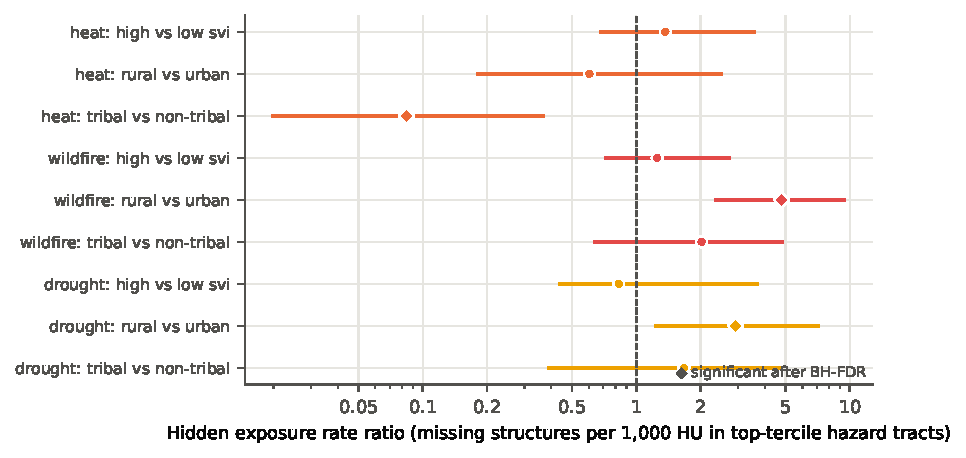
\includegraphics[width=\columnwidth]{fig7_hidden_exposure.pdf}
\caption{Hidden-exposure rate ratios (H5). Diamonds mark contrasts surviving the Benjamini--Hochberg correction.}\label{fig:he}
\end{figure}

\begin{table*}[t]\centering\footnotesize
\caption{All \NFdrFamily{} pre-registered confirmatory contrasts. RD: risk difference; aOR: region-adjusted odds ratio; RR: hidden-exposure rate ratio; $\Delta$: difference in completeness change (H3a) or gap-rate change (H3b); $p_{BH}$: Benjamini--Hochberg adjusted.}\label{tab:conf}
\resizebox{\textwidth}{!}{\begin{tabular}{lllllrrc}
\toprule
Hyp. & Layer & Contrast & Group values & Estimate [95\% CI] & $p$ & $p_{BH}$ & Sig. \\
\midrule
H1 & Bldg & SVI Q4 vs Q1 & 6.0\% / 5.1\% & RD +0.009 [-0.010, +0.025]; aOR 1.19 & 0.278 & 0.535 &  \\
H1 & Bldg & CVI top vs bottom & 6.3\% / 4.5\% & RD +0.018 [-0.005, +0.035]; aOR 1.25 & 0.210 & 0.438 &  \\
H2 & Bldg & Rural vs urban & 5.0\% / 5.2\% & RD -0.002 [-0.022, +0.019]; aOR 1.06 & 0.765 & 0.822 &  \\
H2 & Bldg & Tribal vs non-tribal & 4.2\% / 5.3\% & RD -0.011 [-0.033, +0.013]; aOR 1.12 & 0.850 & 0.850 &  \\
H1 & POI & SVI Q4 vs Q1 & 3.8\% / 8.9\% & RD -0.051 [-0.071, -0.034]; aOR 0.41 & 0.000 & 0.000 & \checkmark \\
H1 & POI & CVI top vs bottom & 4.0\% / 7.5\% & RD -0.035 [-0.053, -0.019]; aOR 0.58 & 0.000 & 0.003 & \checkmark \\
H2 & POI & Rural vs urban & 3.7\% / 5.8\% & RD -0.021 [-0.034, -0.009]; aOR 0.56 & 0.001 & 0.003 & \checkmark \\
H2 & POI & Tribal vs non-tribal & 4.9\% / 5.4\% & RD -0.005 [-0.025, +0.012]; aOR 0.84 & 0.530 & 0.663 &  \\
H5 heat & Bldg & SVI Q4 vs Q1 & 1.41 / 1.03 & RR 1.37 [0.69, 3.54] & 0.313 & 0.559 &  \\
H5 heat & Bldg & Rural vs urban & 0.77 / 1.27 & RR 0.60 [0.18, 2.49] & 0.508 & 0.663 &  \\
H5 heat & Bldg & Tribal vs non-tribal & 0.11 / 1.29 & RR 0.08 [0.00, 0.36] & 0.001 & 0.003 & \checkmark \\
H5 wildfire & Bldg & SVI Q4 vs Q1 & 1.22 / 0.97 & RR 1.25 [0.72, 2.70] & 0.417 & 0.582 &  \\
H5 wildfire & Bldg & Rural vs urban & 3.19 / 0.67 & RR 4.79 [2.38, 9.41] & 0.001 & 0.003 & \checkmark \\
H5 wildfire & Bldg & Tribal vs non-tribal & 1.99 / 0.98 & RR 2.02 [0.64, 4.79] & 0.206 & 0.438 &  \\
H5 drought & Bldg & SVI Q4 vs Q1 & 0.86 / 1.04 & RR 0.83 [0.44, 3.65] & 0.776 & 0.822 &  \\
H5 drought & Bldg & Rural vs urban & 1.78 / 0.61 & RR 2.92 [1.23, 7.13] & 0.014 & 0.044 & \checkmark \\
H5 drought & Bldg & Tribal vs non-tribal & 1.26 / 0.75 & RR 1.67 [0.39, 4.67] & 0.419 & 0.582 &  \\
H3a & Bldg & SVI Q4 vs Q1 & 0.065 / 0.055 & $\Delta$ +0.010 [-0.054, +0.074] & 0.765 & 0.822 &  \\
H3a & Bldg & Rural vs urban & 0.119 / 0.059 & $\Delta$ +0.060 [+0.013, +0.106] & 0.011 & 0.040 & \checkmark \\
H3a & Bldg & Tribal vs non-tribal & 0.079 / 0.069 & $\Delta$ +0.036 [+0.002, +0.070] & 0.038 & 0.095 &  \\
H3a & Bldg & CVI top vs bottom & 0.086 / 0.050 & $\Delta$ +0.038 [-0.045, +0.121] & 0.373 & 0.582 &  \\
H3b & Bldg & SVI Q4 vs Q1 & -- & $\Delta$ -0.006 [-0.052, +0.059] & 0.789 & 0.822 &  \\
H3b & Bldg & CVI top vs bottom & -- & $\Delta$ -0.036 [-0.108, +0.047] & 0.340 & 0.567 &  \\
H3b & Bldg & Rural vs urban & -- & $\Delta$ -0.099 [-0.153, -0.055] & 0.001 & 0.003 & \checkmark \\
H3b & Bldg & Tribal vs non-tribal & -- & $\Delta$ -0.067 [-0.143, -0.006] & 0.022 & 0.061 &  \\
\bottomrule
\end{tabular}}
\end{table*}

\subsection{Catch-up, and a release that went backwards}
Between 2023 and 2026 the share of tracts below 80\% of the reference fell from \GapShareA{} to \GapShareB{}; among rural tracts it fell from \GapRuralA{} to 4.2\%. Rural tracts improved \DidRuralPP{} percentage points more than urban ones ($p_{BH}=\DidRuralP{}$), and tribal tracts \DidTribalPP{} points more ($p_{BH}=\DidTribalP{}$), while the OpenStreetMap share of buildings rose from \OsmShareA{} to 51\% (Fig.~\ref{fig:catch}). The map has caught up fastest where it was furthest behind.

There is one exception. From release \texttt{2026-09-23.0}, Overture dropped about \EOneLost{} buildings, mostly Microsoft-derived footprints, from \EOneTracts{} tracts. Of these, \EOneBexar{} are in Bexar County, Texas; they house \EOneResidents{} people, and \EOneSviShare{} of them are high-SVI tracts, against \EOneSviAll{} across the study area (Fig.~\ref{fig:bexar}). The release notes do not mention the loss.

Re-run on the October release with no reference, the model flagged \EOneFlagAfter{} of the affected tracts, up from \EOneFlagBefore{} before the drop and against \EOneFlagOther{} elsewhere in the region (recall \EOneRecall{}). Monitoring releases for such losses is the application this method supports most strongly.

\begin{figure*}[t]\centering
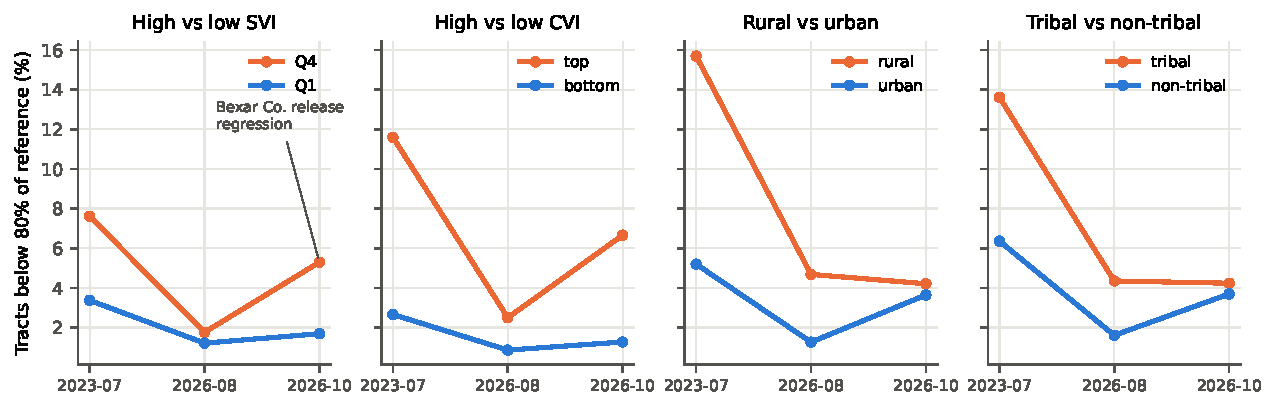
\includegraphics[width=0.9\textwidth]{fig6_catchup.pdf}
\caption{Share of tracts below 80\% of USA Structures by group and snapshot. The 2026-10 uptick is the Bexar County regression, not real-world change.}\label{fig:catch}
\end{figure*}

\begin{figure}[t]\centering
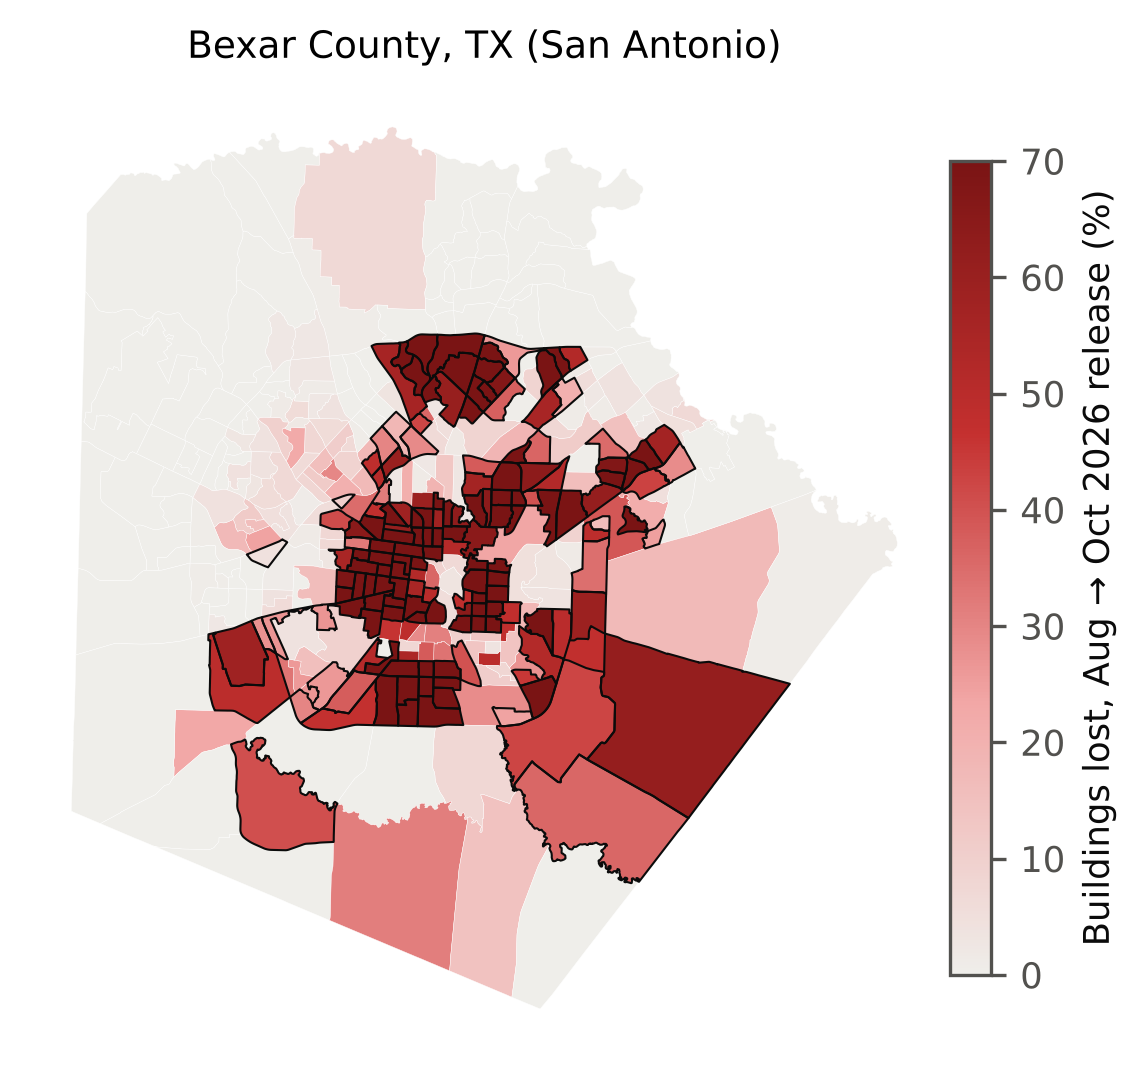
\includegraphics[width=0.85\columnwidth]{fig8_bexar_regression.png}
\caption{Buildings lost between the 2026-08 and 2026-10 releases, Bexar County, Texas.}\label{fig:bexar}
\end{figure}

\subsection{Why per-tract flags miss group-wide gaps}\label{sec:lens}
Measured against the reference, rural tracts have gaps far more often than urban ones (adjusted odds ratio 3.86 [2.40, 6.22]). The model's flag gives 1.06 [0.72, 1.57], and even a reference-anchored flag gives 0.83 [0.48, 1.44]. Tribal tracts show the same pattern: 4.17 [1.89, 9.23] by the reference and 1.26 [0.38, 4.20] by the flag (Fig.~\ref{fig:lens}). Two mechanisms explain this, and neither is an implementation error.

\emph{Absorption.} The expectation is trained on the map, so it learns the rural shortfall as normal. Relative to the reference, observed rural completeness is lower by $-0.031$ [$-0.053$, $-0.009$] log points, and the map-trained expectation is already lower by $-0.025$ [$-0.053$, $+0.004$], reproducing 80\% of the rural shortfall and 64\% of the tribal one.

\emph{Resolution.} Even when anchored on the reference, the tract-level residual SD is 0.21 log points (0.19 for the map-trained model), against 0.22 for a 20\% gap. The noise is therefore as large as the effect to be detected.

Per-tract flags are therefore triage signals, and equity claims require reference comparisons aggregated by group.

\begin{figure}[t]\centering
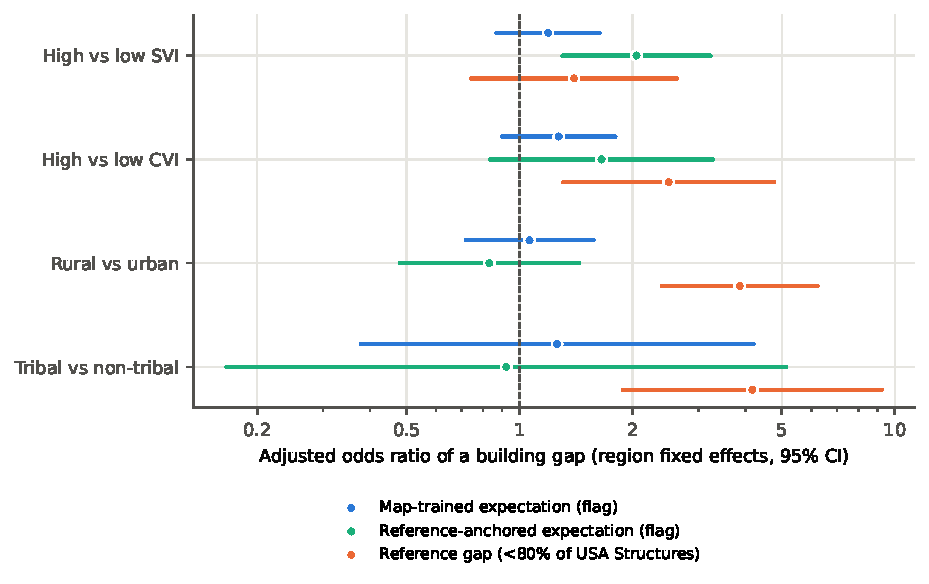
\includegraphics[width=\columnwidth]{fig5_two_lenses.pdf}
\caption{Odds ratios of a building gap by group under three lenses: the map-trained flag, a reference-anchored flag, and the reference gap itself.}\label{fig:lens}
\end{figure}

\subsection{Baselines, imports and robustness (exploratory)}
We tested whether the conformal model is needed for ranking. Under an identical budget of \MgBudget{} flags, eight methods, including an Isolation Forest on log counts, reach \MgLiftMin{}$\times$--\MgLiftMax{}$\times$ lift against 1.0$\times$ for random flags, and none differs from the conformal model in precision, recall or PR-AUC under a paired county-cluster bootstrap (Table~\ref{tab:baselines}). The method's contribution is therefore calibrated ranges and release monitoring, not better ranking.

\begin{table}[t]\centering\footnotesize
\caption{Exploratory: eight methods under one budget of \MgBudget{} flags, scored against the USA Structures gap (prevalence \PrevBldg{}). None differs significantly from the conformal model.}\label{tab:baselines}
\resizebox{\columnwidth}{!}{\begin{tabular}{lrrrrr}\toprule
Method & Precision & Recall & Lift & ROC-AUC & PR-AUC\\\midrule
Conformal model (this paper) & 0.094 & 0.264 & 5.06 & 0.685 & 0.099\\
Isolation Forest on log counts & 0.098 & 0.275 & 5.28 & 0.766 & 0.095\\
NB GLM shortfall & 0.094 & 0.264 & 5.06 & 0.736 & 0.069\\
Map/housing ratio & 0.090 & 0.253 & 4.85 & 0.463 & 0.081\\
XGBoost shortfall & 0.086 & 0.242 & 4.64 & 0.730 & 0.071\\
OLS on housing units and area & 0.075 & 0.209 & 4.01 & 0.729 & 0.063\\
XGBoost, structure + rural + region & 0.075 & 0.209 & 4.01 & 0.686 & 0.064\\
\quad + neighbours' building density & 0.075 & 0.209 & 4.01 & 0.670 & 0.066\\
Random flags (1,000 draws) & 0.019 & 0.053 & 1.01 & 0.500 & 0.019\\
\bottomrule\end{tabular}
}
\end{table}

Machine-learned imports fail in two ways. They can be withdrawn: \MgRegMsftPooled{} of the buildings lost in Bexar County were Microsoft-derived. Where they remain, they lack attributes: in the \MgDomTracts{} tracts that are at least 90\% Microsoft footprints, only \MgDomLabel{} of buildings carry a use class, against \MgOtherLabel{} elsewhere. Consistent with this, reference gaps are more common in Microsoft-dominated tracts (2.8\%) than in OSM-dominated ones (1.3\%).

Robustness: across 7 specifications (primary; no housing-type covariates; negative-binomial GLM; 80\% and 95\% ranges; within-region calibration; excluding tracts under 50 housing units), 53 of 56 flag contrasts keep their significance status. The lower POI flag rate in high-SVI tracts holds in every one (RD $-0.040$ to $-0.067$). The main exception is informative: dropping units-in-structure covariates makes building flags significantly more common in high-SVI tracts (aOR 2.91). This is consistent with absorption, because mobile-home and multi-unit shares correlate with SVI and, in the primary model, explain part of the high-SVI shortfall.

Across \MgNVariants{} model settings, coverage stays at \MgCovMin{}--\MgCovMax{}. Individual flags are less stable: changing only the random seed leaves a flag-set overlap of \MgSeedOverlap{}, and across ten seeds the overlap is \JsPairMin{}--\JsPairMax{}. The \JsStable{} tracts flagged under at least nine seeds are more precise (lift \JsStableLift{}$\times$), which supports reporting a seed-stable core rather than a single run.

Two further checks support these findings. A one-sided 5\% lower bound, which matches the one-directional flag, flags \JoFlagRate{} of tracts and selects nearly the same set (Jaccard \JoJaccard{}). Measured directly against the reference, missing structures in high-wildfire rural tracts are \JhWildfireRural{}$\times$ more common, well above the model-based \HFiveWildRural{}$\times$, which again indicates absorption.

\section{Deviations From the Plan}
We record four deviations. We targeted five whole states and Overture \texttt{2025-09-24.0}; Overture deletes releases after about 60 days and the strata are distributed for the challenge regions, so we used those regions and the three snapshots that could be obtained. The Phase~1 gate found only \RefGapShare{} of tracts below 80\% of the reference, a weaker signal than assumed, so we report both layers rather than buildings alone. LODES jobs were added because ACS alone explained only $R^2=0.42$ of POI variance. And rurality is RUCA $\geq 4$ throughout, as pre-registered, not the Census urban/rural class; under the Census class the rural reference excess is 2.64$\times$ rather than \RvRuralRef{}$\times$.

\section{Limitations}
\emph{From the data:} both building sources are imagery-derived, so a shared omission would make us understate gaps; the POI reference counts employer establishments allocated by land area, so POI validation is approximate; hazards are tract averages, so hidden exposure assumes missing structures share their tract's hazard; the 2023 snapshot is a third-party archived alpha release; \RvN{} of the \NTracts{} tracts carry a usable reference count, one having none and five fewer than ten reference buildings; and five hazard-selected regions are not a national sample.

\emph{From our own checks:} single-tract flags move with the random seed (overlap \MgSeedOverlap{}), so they are triage signals rather than verdicts; calibration is uneven by tract size, with \MgFlagSmallDecile{} of the smallest expected-size decile flagged against \MgFlagLargeDecile{} of the largest, so the 90\% guarantee holds on average rather than everywhere; USA Structures imagery dates from \MgImgFirst{}--\MgImgLast{}, so recent construction or demolition blurs the comparison; ACS margins of error are ignored, which matters most for the \MgGqTracts{} tracts that are mostly group quarters; residuals stay spatially autocorrelated within regions (Moran's $I$ \MgMoranMin{}--\MgMoranMax{}); and eastern Washington is almost never flagged (\MgWaFlag{}).

\section{Conclusion}
A reference-free conformal model can audit an open map with calibrated uncertainty, detect real losses between releases, and link the gaps it finds to hidden climate exposure. Its flag rate is calibrated against the map's own distribution, which is not the same as a known false-alarm rate against the truth, and a 50\% loss is caught in \DelFiftyBldg{} of tracts.

Two recommendations follow. First, per-tract flags should be paired with group-level reference comparisons whenever the question concerns equity, because a gap shared by a whole group is nearly invisible to a per-tract test. Second, release monitoring is the strongest use case: open-map releases change every few weeks, and they are not routinely checked for losses. Next steps are national release-regression monitoring, checking whether the San Antonio buildings return, and group-level audits for roads and emergency facilities.

\bibliographystyle{IEEEtran}
\bibliography{../../paper/refs}
\end{document}
